
\say{To ensure good quality global CAA solutions, the outer boundaries of the computational domain must be transparent to all outgoing waves} - \textcite{tam193DRP}


Generally speaking, within computational aeroacoustics there are a number of categories for solving sound problems. Firstly there are the acoustic analogies / integral approaches (Lighthill's analogy \cite{lighthill1952onsoundsgenerated}, Ffowcs Williams-Hawkings analogy \cite{ffowcswilliams1969soundgenerationturb}, Curle analogy \cite{curle1955influencesolid}, Kirchhoff-Helmholtz integral \cite{godin1996kirchhoffhelmholtz}), where the propagation of acoustics into the far field is calculated from knowing the flow field variables near the source. Secondly there is the hybrid approach (\textcite{hardin1994acousticsplitting}, \textcite{shen1999commentpopeformulation}, \textcite{ekaterinaris1999newformulationhardinpope}) where the computational domain is decoupled into a flow field and acoustic field so that differing equations and numerical methods can be used to solve for each sub-domain (which vary substantially in scale). The flow field is achieved through a standard CFD solver using either steady-state (RANS) or transient (LES, DES, URANS) solutions. The noise source terms are extracted from the mean flow field\footnote[1]{this is a vast oversimplification, however, a noise source investigation is beyond the scope of this project} and then fed to an acoustic propagation solver. Thirdly there is the linear and nonlinear wave propagation approach using finite difference schemes, which covers a large area of the CAA research space (\textcite{tam2012computational}, \textcite{zingg1996reviewFD}, \textcite{kubratskii2004reviewcaaalgo}). With this approach, partial differential equations (PDEs) describing wave propagation are discretised in space and time to resolve large bandwidths of wavenumbers\footnote[2]{wavenumber being the spatial equivalent of a wave's frequency} with minimal error. Lastly, there is a batch of alternative methods including: lattice gas automata (LGA) \cite{doolen1991LGM}, finite element methods (FEM) \cite{peyret2001FEMCAA}, and boundary element methods (BEM) \cite{kirkup2019BEMCAA} - which are less common within CAA. The third approach of finite difference schemes for linearised governing equations is to be used for this project - as this offers the greatest flexibility in terms of investigating novel boundary conditions.


Acoustic problems as presented in the context of this project are typically within unbounded domains in real-life. Simulating these problems computationally requires the domain to be bounded or truncated. Within typical open-domain CFD problems, the subject of boundary conditions is trivial - the farfield is set far enough away from the body/geometry to remove interference and any propagating flow phenomena are simply dissipated throughout the domain farfield. When considering aeroacoustics, low-dispersion, low-dissipation methods are required which allow for waves to propagate for very large distances within the domain. Therefore, it is important for boundary conditions to be integrated which allow for the waves to outflow through the domain boundaries without affecting the inner domain, to be able to constrain the problem to a sensible size. Otherwise, the computational effort required for a solution with a far enough boundary to avoid reflections is nonsensical. The solution is to implement non-reflecting boundary conditions (NRBC), as illustrated by Figures \ref{fig:UnboundedDomain} and \ref{fig:TruncatedDomain}.


\begin{figure}[h]
    \centering
    \begin{subfigure}[h]{0.47\textwidth}
        \centering
        \makebox[0pt]{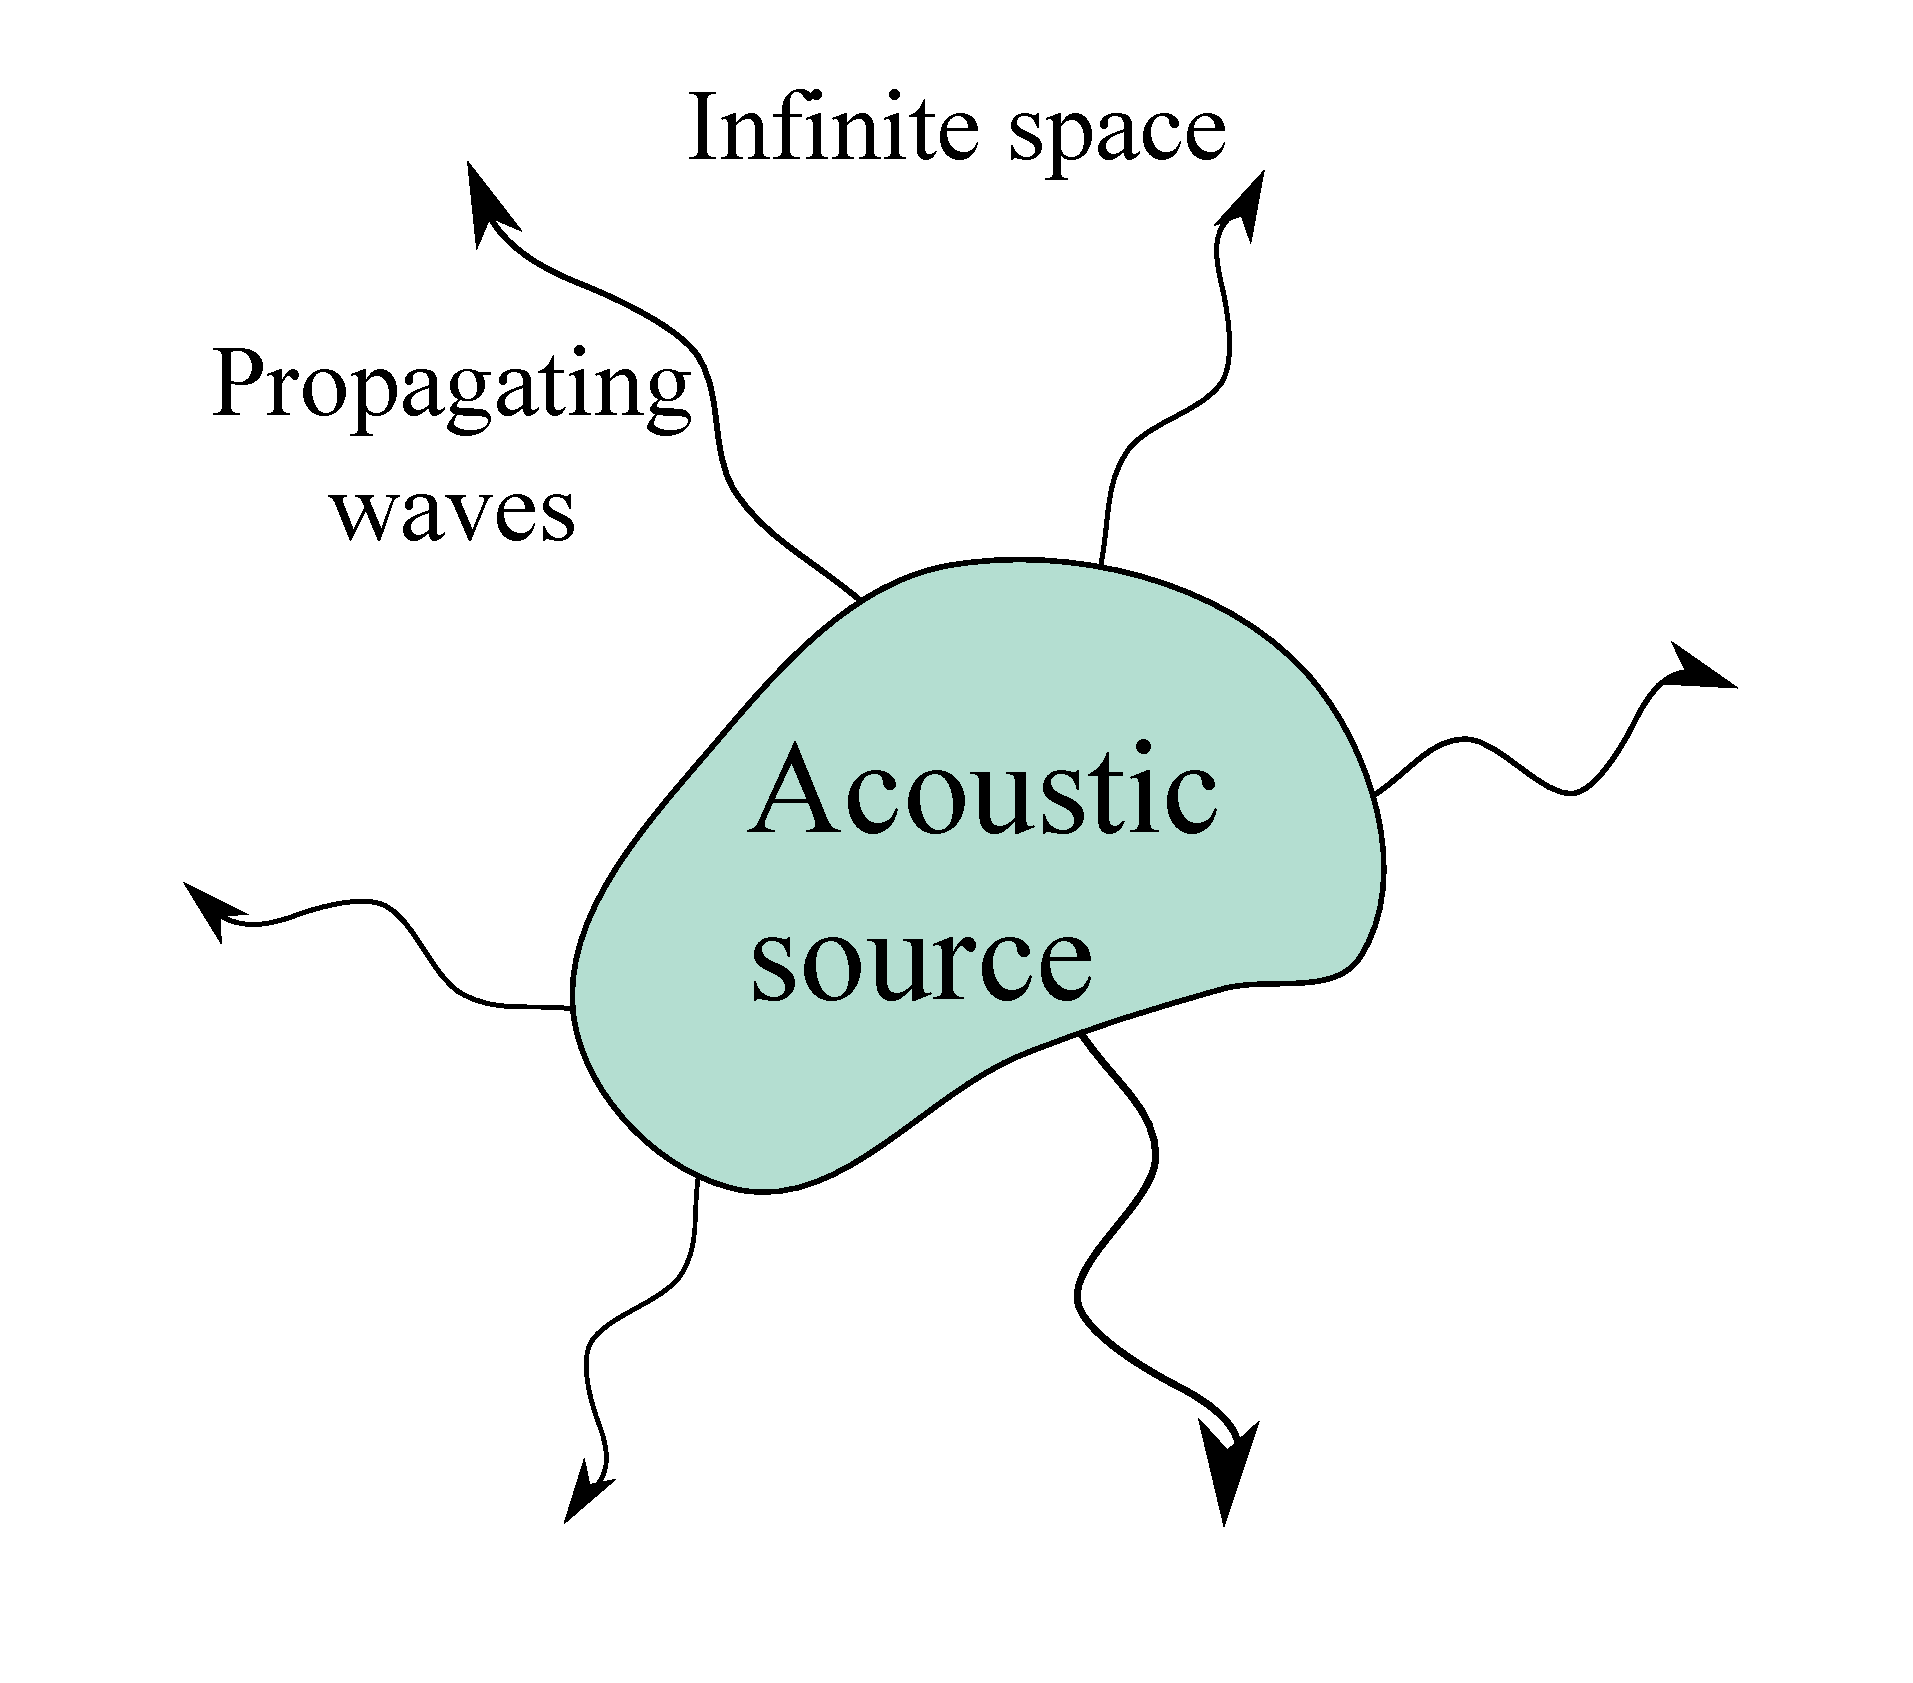
\includegraphics[width=7cm]{Figures/IntroBackground/UnboundedRegion.eps}}
        \caption{}
        \label{fig:UnboundedDomain}
    \end{subfigure}
    \hfill
    \begin{subfigure}[h]{0.47\textwidth}
        \centering
        \makebox[0pt]{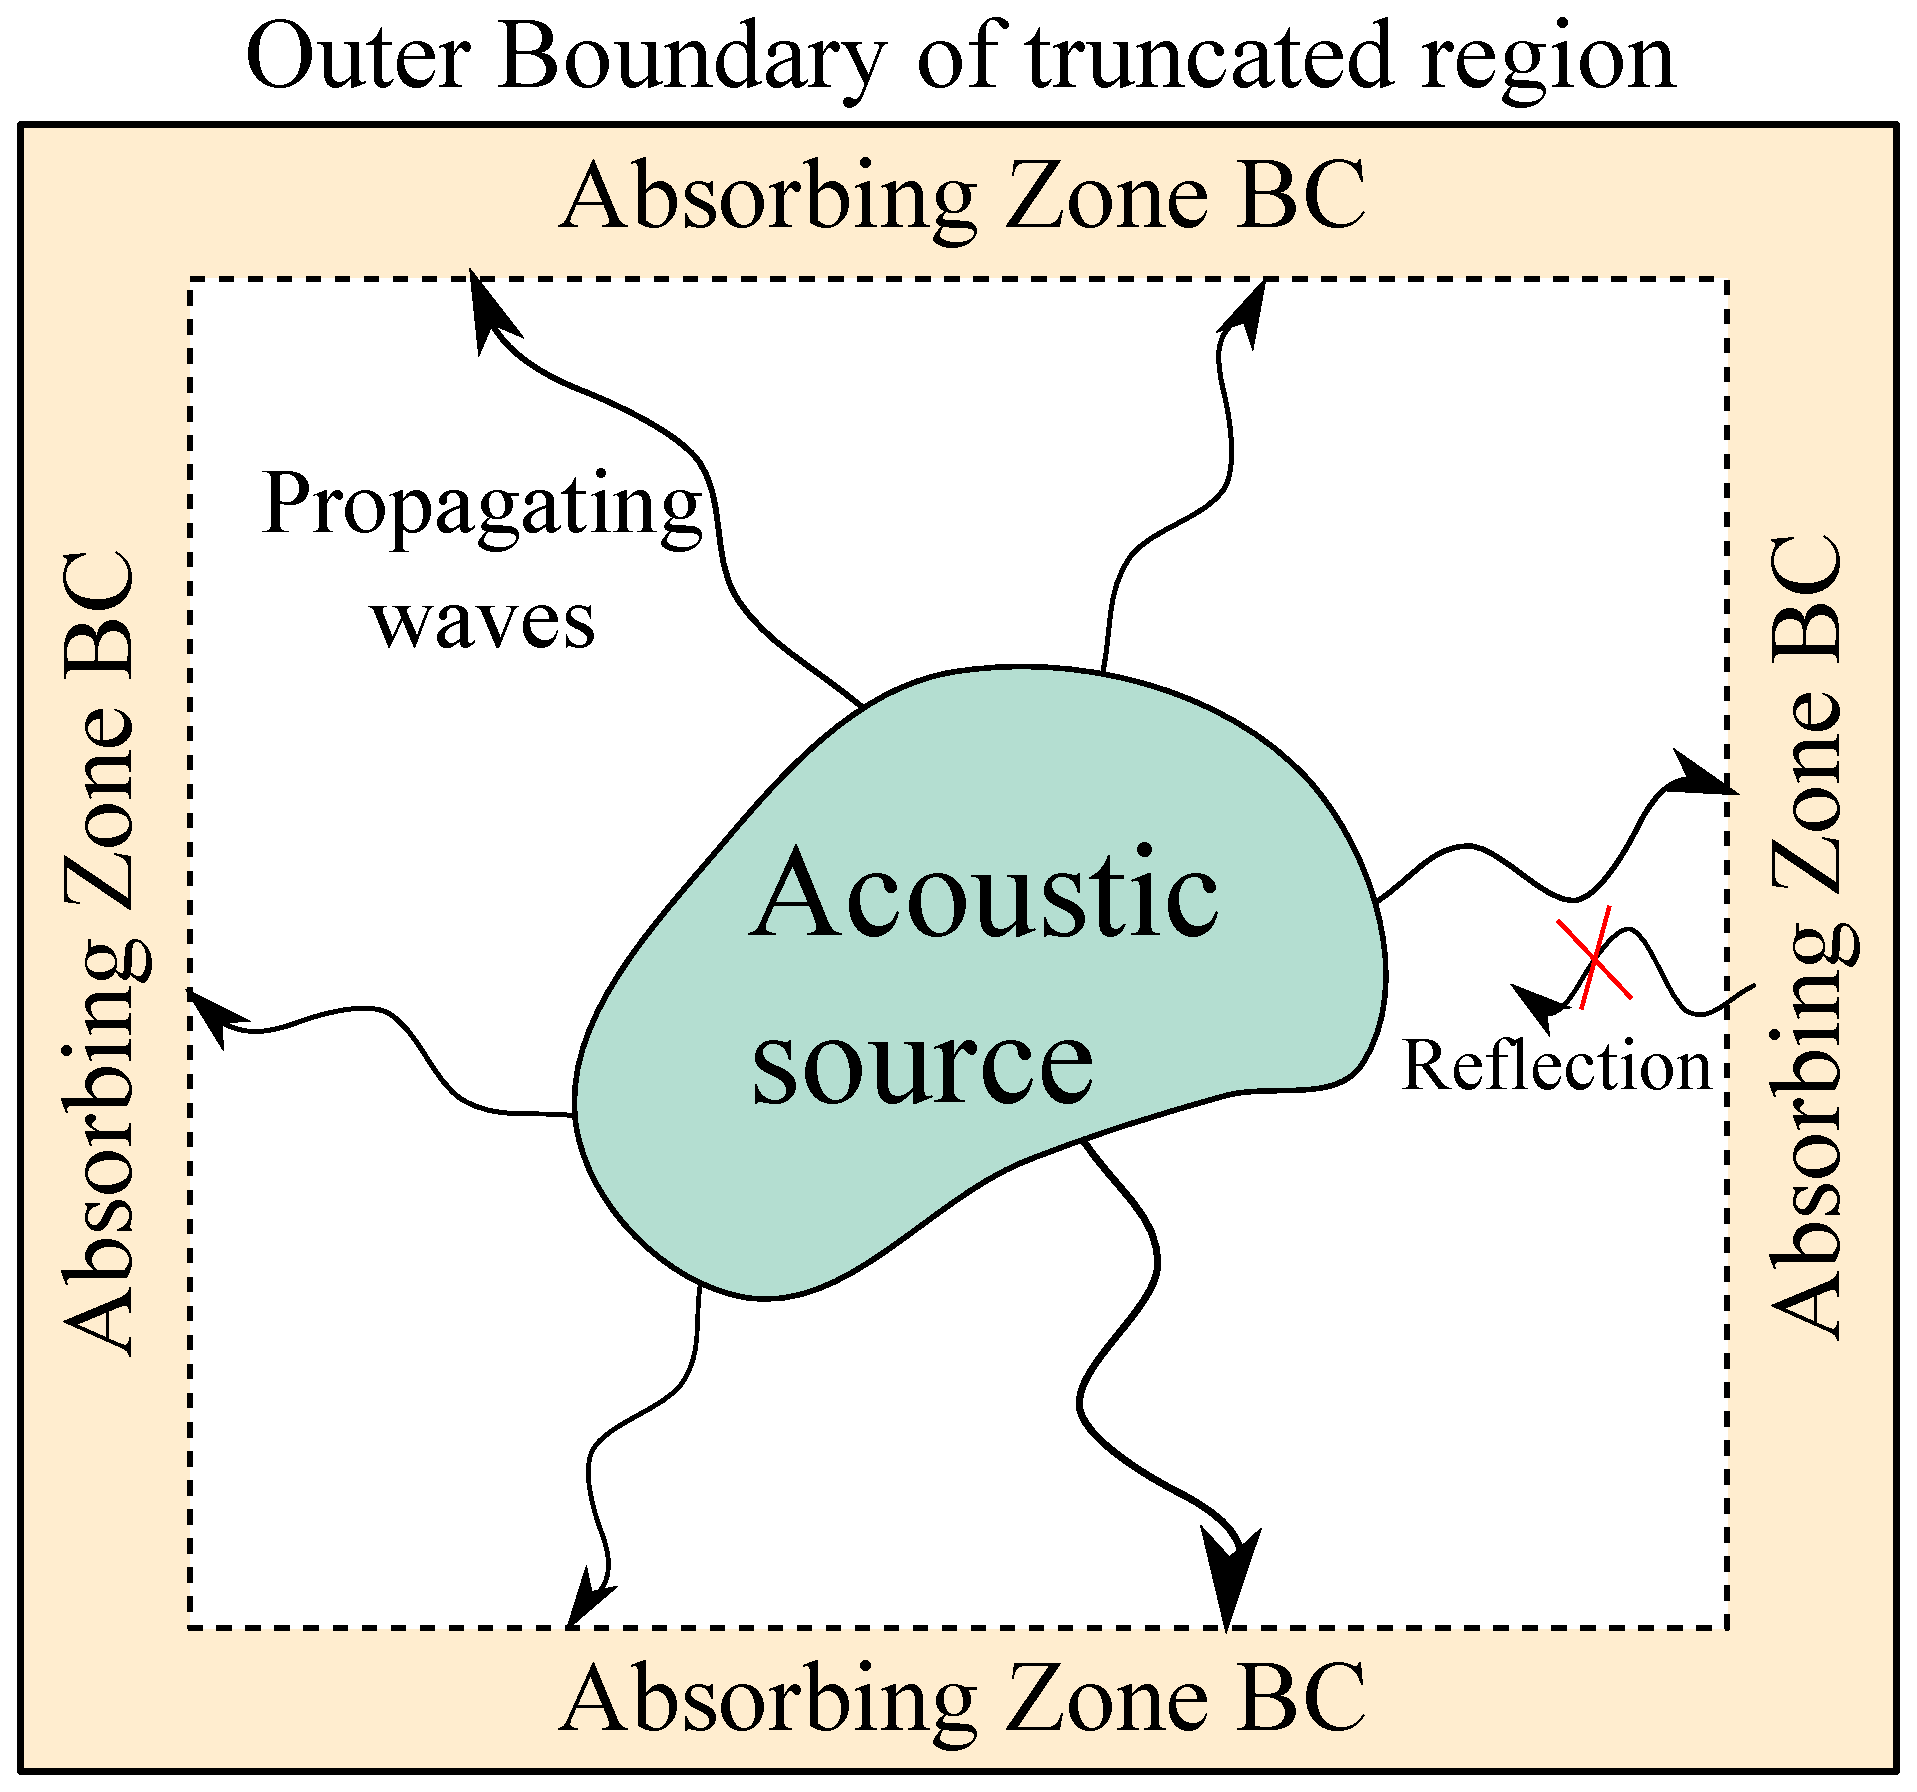
\includegraphics[width=7cm]{Figures/IntroBackground/TruncatedRegion.eps}}
        \caption{}
        \label{fig:TruncatedDomain}
    \end{subfigure}
    \caption{Simplified solution space, with a finite inner region of interest containing an acoustic source. (\textbf{a}) shows propagating waves extending to infinity, and (\textbf{b}) shows a truncated region with an absorbing zone boundary condition where propagating waves are damped to inhibit reflections \& error in the inner domain.}
    \label{fig:Domain}
\end{figure}


\textcite{kim2000generalizedcharbc} group NRBC's into 3 main types. The first are formulations based on the characteristic directions of governing equations, but these are quickly dismissed for the CAA application due to the ineffectiveness for waves impinging on the boundary at any varying angle, as described by \textcite{colonius2004modelling}. The second are formulations based on the asymptotic solution of the governing equations, where the equations are solved in the farfield for a uniform flow. \textcite{bayliss1982farfield} conclude that the asymptotic BC requires the farfield be placed sufficiently far to achieve accuracy comparable to other BCs mentioned here. This increases the computational cost and hazes the applicability with regards to what domain size is suitable. The final type of NRBC are formulations based on damping/buffer/sponge zones being added to the boundary, where the incident waves are filtered/stretched/damped to prevent reflections. This type of NRBC is by far the most applicable and does not depend on the flow characteristics - as the first type does.

There are a number of damping zone non-reflecting boundary conditions that have been formulated for methods which solve both linearised and nonlinearised Euler equations. Three have been identified from literature as potential solutions.
The PML method, originally derived as a solution for Maxwell's equations by \textcite{berenger1994apml} and adapted for aeroacoustics by \textcite{hu1996onabsorbingbc} \cite{hu2001astablePML} \cite{hu2005aPML}, is a strong version of the damping zone NRBC which absorbs out-flowing waves at domain boundaries by constructing modified governing equations (differently to the earlier NRBCs) with an additional dissipation term. The original aeroacoustic formulation was plagued by numerical instability, but was later amended in \cite{hu2005aPML} by aligning the group and phase velocities using a space-time transformation.

A second formulation of damping zone NRBC is the Buffer Zone (BZ), formulated by \textcite{wasitho1997simulationtfsei}, which is in fact very similar to the PML NRBC where the out-flowing waves in the buffer zone are damped as determined by a damping function. The exact formulation and method of numerical damping is slightly different to the PML and is an effective NRBC in its own right.


The final formulation of damping zone NRBC is the Energy Transfer and Annihilation (ETA), formulated by \textcite{edgar2012generalbufferzone}, which is based on stretching and filtering of the grid. As in, the energy content of the waves entering the NRBC is transferred to higher wavenumber waves using stretching of the grid. These are then subsequently eliminated using high-order numerical filtering which targets the higher wavenumbers.


\textcite{manco2019comparativesnrbc} make comparisons between the NRBC's for three different flow problems: linearised Euler equations in uniform flows, linearised Euler equations in non-uniform flows, and nonlinear Euler equations for mixing layer-type flows. For simplification, the project will opt with the linearised Euler equations in uniform flow case. The author concludes that the ETA NRBC is not as accurate as the PML or BZ - and supports more reflections as the wavefront propagates towards the boundary. The PML and BZ are reported to be very evenly matched when instantiated with similar parameters, and also happen to compute in similar CPU times. Given the application and prevalence of the PML in literature, it is the chosen NRBC.

On the topic of PML application, it's use is apparent throughout wave-type problems - both in research and in industry. For example, in electromagnetics it has been used for modelling marine controlled source electromagnetics to map ocean subsurface topology (\textcite{li2017marineCSEM}), and in aeroacoustics it has been used for developing an adjoint CAA solver for optimising acoustic liners (\textcite{ozkaya2016adjointcaaliner}). Typically, any mention of setting 'optimal' PML parameters is scarce, and where it has been mentioned, it is hastily handled by setting very large widths effectively dismissing potential efficiency gains.


Within current literature, there exists 4 papers which explore optimisation of PML performance \cite{choung2018nonreflective}\cite{li2003optimizationPML}\cite{margengo1999optimumpml}\cite{agrawal2004pmlperformance}. The latter 3 of which look to investigate the effects of the PML parameters via numerical means, albeit considering them exclusively - disregarding the relationship between damping coefficient and PML width. These 3 papers also originate in the late 1990's / early 2000's and are solely concerned with elastodynamics and electromagnetics, decreasing their relevance for the suggested application due to differing governing equations and domain setup. The first paper \cite{choung2018nonreflective} is the most recent (and only) piece of research to analytically optimise the PML parameters. The researchers assume that there are two factors inducing error within the domain: spurious waves from too small of a PML, causing discontinuous damping, and spurious waves from too little damping (defined by the coefficient), so that waves are not fully decayed by the end of the PML. These factors are proven to be intrinsically linked in that a change in one parameter might mean the other could be smaller/more efficient (e.g. the same damping coefficient might be suitable for a thicker PML, but produces errors for a thinner PML). 

One drawback of the analytical derivation \cite{choung2018nonreflective} is the underlying assumption that the induced error is only caused by two factors, which implies the mechanisms and interactions of the PML BC with the domain are fully understood to the letter\footnote[1]{one might be dubious to this fact}. This leads on nicely to \textit{numerically} optimising the PML parameters in this project through design sweeps, knowing there is a source of published analytical optimums to contrast and compare against. This project is mainly focused on optimising the PML performance, not necessarily comparing it to other boundary conditions in its effectiveness.

It should be noted that at the time of writing, \cite{choung2018nonreflective} is yet to be cited and so the resultant optimal conditions have not been formally used in a CAA solver implementing PML boundary conditions.


\textbf{Literature review findings:}
\begin{itemize}
    \itemsep0em
    \item Characteristic, asymptotic, and damping zone non-reflecting boundary conditions for CAA
    \item 3 damping zone non-reflecting boundary conditions (Perfectly Matched Layer, Buffer Zone, Energy Transfer and Annihilation) which outperform characteristic and asymptotic BCs
    \item 4 papers exploring optimisation of PML performance
    \item 1 out of the 4 is concerned with aeroacoustics, and considers all the parameters inclusively
    \item Only analytical methods were used in the paper to find optimal PML conditions, opening a door for numerical methods in this project
\end{itemize}
